\chapter{Background}

This chapter describes some background information on Approximate Computing and the automated framework IIDEAA. Section on Approximate Computing will cover its definition, motivation, challenges, and some basic strategies. As for IIDEAA, we will present two tools that the framework is made up of: Clang-Chimera, a source-to-source mutation software that apply pre-defined code mutator corresponding to some of the strategies. The other tool is an Evolution search engine named Bellerophon, which goes through Chimera's mutated source code to find the best approximated version of the program, based on how the user decide to calculate the error, reward and penalty functions. Also, some state of the art regarding automation for Approximate Computing will be introduced as well.\\

\section{Approximate Computing}

\subsection{Motivation}

Approximate computing is a computational technique that loosen up the accuracy requirement of mathematical operations performed by computers, returning a result that is possibly inaccurate (but not incorrect) compares to the exact result, yet is still within the range of "acceptable error" for an application to function properly. Such applications that enable Approximate Computing are called "error-tolerant" applications \cite{7348659}. These applications usually have gaps between the accuracy level it(or the user) require and that of the system can deliver, and thus is capitalized by Approximate Computing to produce a variety of optimizations \cite{AxCSurvey}. \\
~\\
By reducing the stress of exact calculation and some minor loss of precision, this technique can promise a gain in efficiency, in terms of speed, memory, energy consumption, etc. As a prime example, the approximated version of k-mean clustering algorithm, tested by Chippa, achieved up to 50x energy reduction while losing only 5\% of accuracy and up to 5x energy reduction with insignificant error \cite{SEHD}.\\
~\\
Approximate Computing can be conducted on both hardware and software layer, providing diverse methods to apply the technique to applications. On hardware level, the target can be either: circuits, by replacing them with less accurate but more energy-efficient one, or the voltage of the hardware component, deliberately lowering it to make a compromise between accuracy and energy-consumption. With software layer, the general strategy is to overlook or reduce parts of the program that have insignificant contribution to the final result \cite{7348659}, such as loop perforation(skipping certain iteration in loop), code perforation(disregard parts that have little impact),precision scaling (reduce the precision of calculation), thread fusion(merging dynamic instances of the same static instruction from different thread into one), etc.\\
~\\
%\subsection{Motivation}
%
Current era computing, while being advanced, is still without its own dilemma. Large-scale applications, namely scientific computing, social media, business and financial analysis drain far too much resources than what is available. A prediction was made that by 2020, datacenters in US will consume about 140 billion kWh of electricity, a huge increase from 91 billion kWh in 2013 \cite{NRDC}. It is clear that while computing applications are achieving incredible performance and results, the amount of resources they require is soon to be out of control as the planet's resources are limited and decreasing everyday \cite{AxCSurvey}. \\
~\\
%One of the main cause of this problem is fault-free computing, which can be usually resource-intensive. The current generation computer circuit's design contains components are more vulnerable to faults and parameter variations due to low voltage supply and ever-growing integration density \cite{1322441}. Thus, for faultless computation to be used, guardbands for protection against parameter variations and error correction is apply, which increase the energy overhead tremendously \cite{7348659}. \\
~\\
Due to this fact, Approximate Computing raises as a potential solution, being the topic of interest in both industry and academic researches \cite{7348659}. Furthermore, many modern days application have inexact or noisy input, limited data precision, or are not able to find an exact output. Consequently, faultless computing becomes more redundant as rounding off results happens more often, making Approximate Computing a more optimal choice \cite{AxCSurvey}. \\

\subsection{Level of Approximate Computing}

In the article "Introduction to Approximate Computing", the author, Ben Khadra, has suggested a structure to classify all forms of development for Approximate Computing. One parameter of classification among the structure presented is the Level of Approximation, indicating which part of the system the technique is applied on. The four following categories were presented from lowest to highest respectively, in terms of cost-effective: algorithm, application, architecture, and circuit \cite{introAxC}. \\
\begin{figure}[H]
%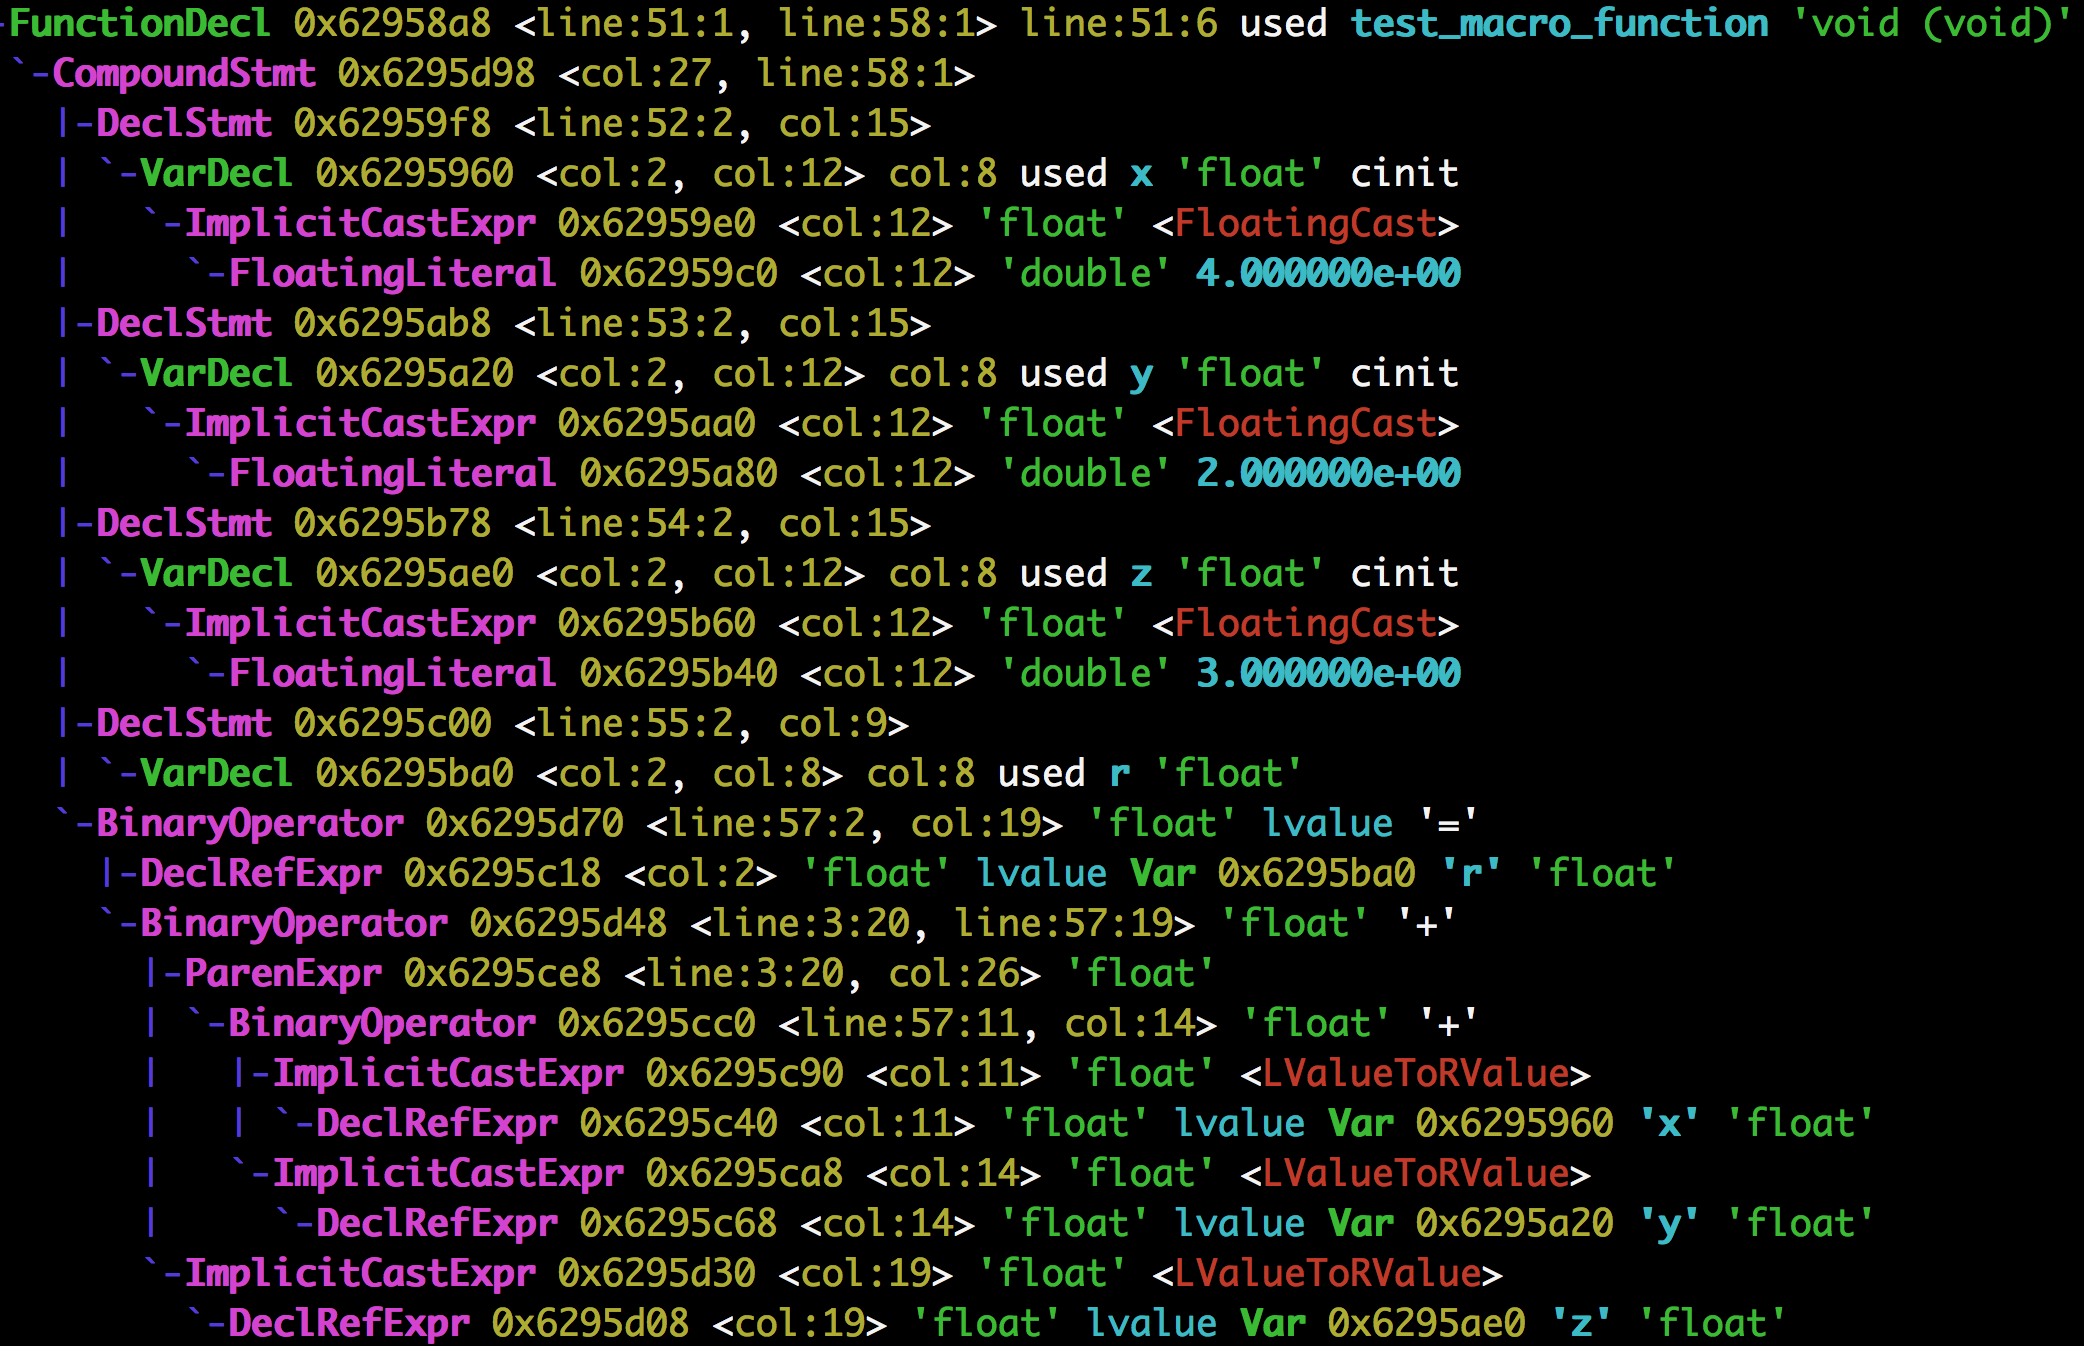
\includegraphics[width=15cm]{ast-sample.png}
\centering
\caption{Level of Approximate Computing}
\end{figure}
~\\
Changes made at algorithm level usually are related to inputs or configuration of the algorithm while not altering the said algorithm. For application level, on the other hand, modifications to the algorithm are required. Another way to apply Approximate Computing at this level is having the ability to inspect a larger search space, for example automating the process to discover many Approximated variants of the application. Higher levels of Approximate Computing typically include adjustments to hardware, with the top-level being circuit modification. At this level, the design of the circuit is the target by changing or adding new arithmetic units, for instance adders and multipliers, which is created for approximate computing. This level is also considered as the most expensive to implement since implementations physically change the circuit into a new one \cite{introAxC}.

\subsection{Common Strategies}

\subsubsection{Precision Scaling}

As the name imply, this strategy focuses on alternating the precision/bit-width of the input or intermediate operations. Precision Scaling is usually used with Floating Point operations, and generally results in a reduction in memory requirement or computational stress. It has been revealed that by decreasing the bit-width, it allow some optimizations can be viable. One of them being reducing Floating Point operations to a much simpler, insignificant operations (such as multiply by 1) which in turns do not require a Floating Point Unit. Another is allowing the use of smaller, much faster Floating Point Unit than the typical Floating Point Unit \cite{4408271}. Moreover, the strategy can also reduce the ammount of data transfer from/to the memory. \\
~\\
While Precision Scaling is mainly applied to hardware layer, more specifically on architechtural level, it can still be used on software level. To perform Precision Scaling on hardware layer, one can target directly the Floating Point Unit, altering its architecture \cite{AxCSurvey}. However the same cannot be said for software layer. Without specific hardware and programming library support, it is almost impossible to do so since programmers are stuck with very basic data type, such as single-precision (32-bit) and double-precision (64-bit) floating point number. \\
~\\
Currently, with the introduction of Pascal GPU Architecture and CUDA8 API, NVIDIA has provided half-precision (16-bit) floating point number data type for computing in lower precision \cite{CUDA8}. Despite not being as in full control nor as flexible as hardware Precision Scaling, the 16-bit floating point number has made Precision Scaling strategy more viable on software level, especially how GPU has been playing an important part in modern High Performance Computing. \\

\subsubsection{Loop Perforation}

Unlike Precision Scaling which can be applied at both hardware layer and software layer, Loop Perforation explicitly targets the software layer, performing Approximate Computing by directly making changes to the application. The strategy reduces computational time(thus reducing resources consumption) by only executing only a major portion of the loop's total iterations while skipping the some of it. Loop Perforation can succeed due to the fact it takes advantage of partially redundant computations that often manifest when processing multiple inputs to acquire one output \cite{LoopPerforation}. \\

\subsection{Challenges}

Like everything that existed, Approximate Computing has its own shortcomings that limit its potential. The most noticeable drawback is the nature of the technique. Because it produces imprecise results, applications that require hard logical correctness to operate as desired are not suited to apply approximation. Examples of those are cryptography, operating system, compiler, etc. Some applications are reported to only have a limited range of input where Approximate Computing is effective \cite{AxCSurvey}. \\
~\\
Excessive use of Approximate Computing may lead to undesired behaviors that cause the program to function incorrectly. It is reported that calculating a matrix kernel with Approximate Computing applied can lead to an unsolvable solution, which blocks the program and prevents its termination \cite{AxCSurvey}. Tested by Akturk \cite{Akturk2015OnQO}, Approximate Computing, in some cases, can generate corrupted output that still passed the chosen quality metric. On top of that, in worse cases, applying the technique may cause interference with the program's synchronization process and memory ordering, and consequently produces non-deterministic results which is hard to debug.\\
~\\
Finding the right strategy for the designated program can be a daunting task. Aside from the 2 basic strategies mentioned above, there are many others to choose from, which vary in terms of scope, cost, flexibility, etc. Picking a optimal methods out of all the existing tactics proves to be difficult since they can cause different experience with different applications, and nothing can work universally. It also depends greatly on requirements and constraints imposed by the user \cite{Ansel}. \\
~\\
Another challenge that Approximate Computing must face today is the lack of automation. Up until now, Approximate Computing has played a part in the advancement of Computer Science, from lossy image compression algorithms to wireless communication. Nevertheless, manually applying this technique based on the past knowledge and experience seemed to be inefficient. Applications complexity has outgrown the 2 fore-mentioned aspects, thus rises the need for (semi)automatic frameworks that can efficiently generate approximate computing system \cite{introAxC}. \\

\section{IIDEAA Automate Framework} 

The IIDEAA framework was developed to tackle one of the challenges that is holding Approximate Computing advancement back: the absence of a general automated tool that can explore a larger possibilities of a given Approximate Computing strategy more proficient and find the best compromise between the level of inaccuracy and the efficient gained in the process. \\
~\\
The main selling point of this open-source framework is that the user does not need to detail which part of the program to be approximated and in what way. It only asks for which functions that need to be approximated and the desired error threshold to find the best possible result. Depending on what approximate strategy is used, the framework can produce a hardware or sofware implementation of the approximated application ~\cite{iideaa}. \\
~\\
IIDEAA comprises of two smaller tools that was written in C++. The first one is Chimera, a source-to-source mutation software that can modify C/C++ source code with a given code mutator. The second tool is called Bellerophon which offers a Evolutionary Search Engine to explore the mutated code to find all the best functional approximated versions that satisfy the user's requirements. \\
\begin{figure}[H]
%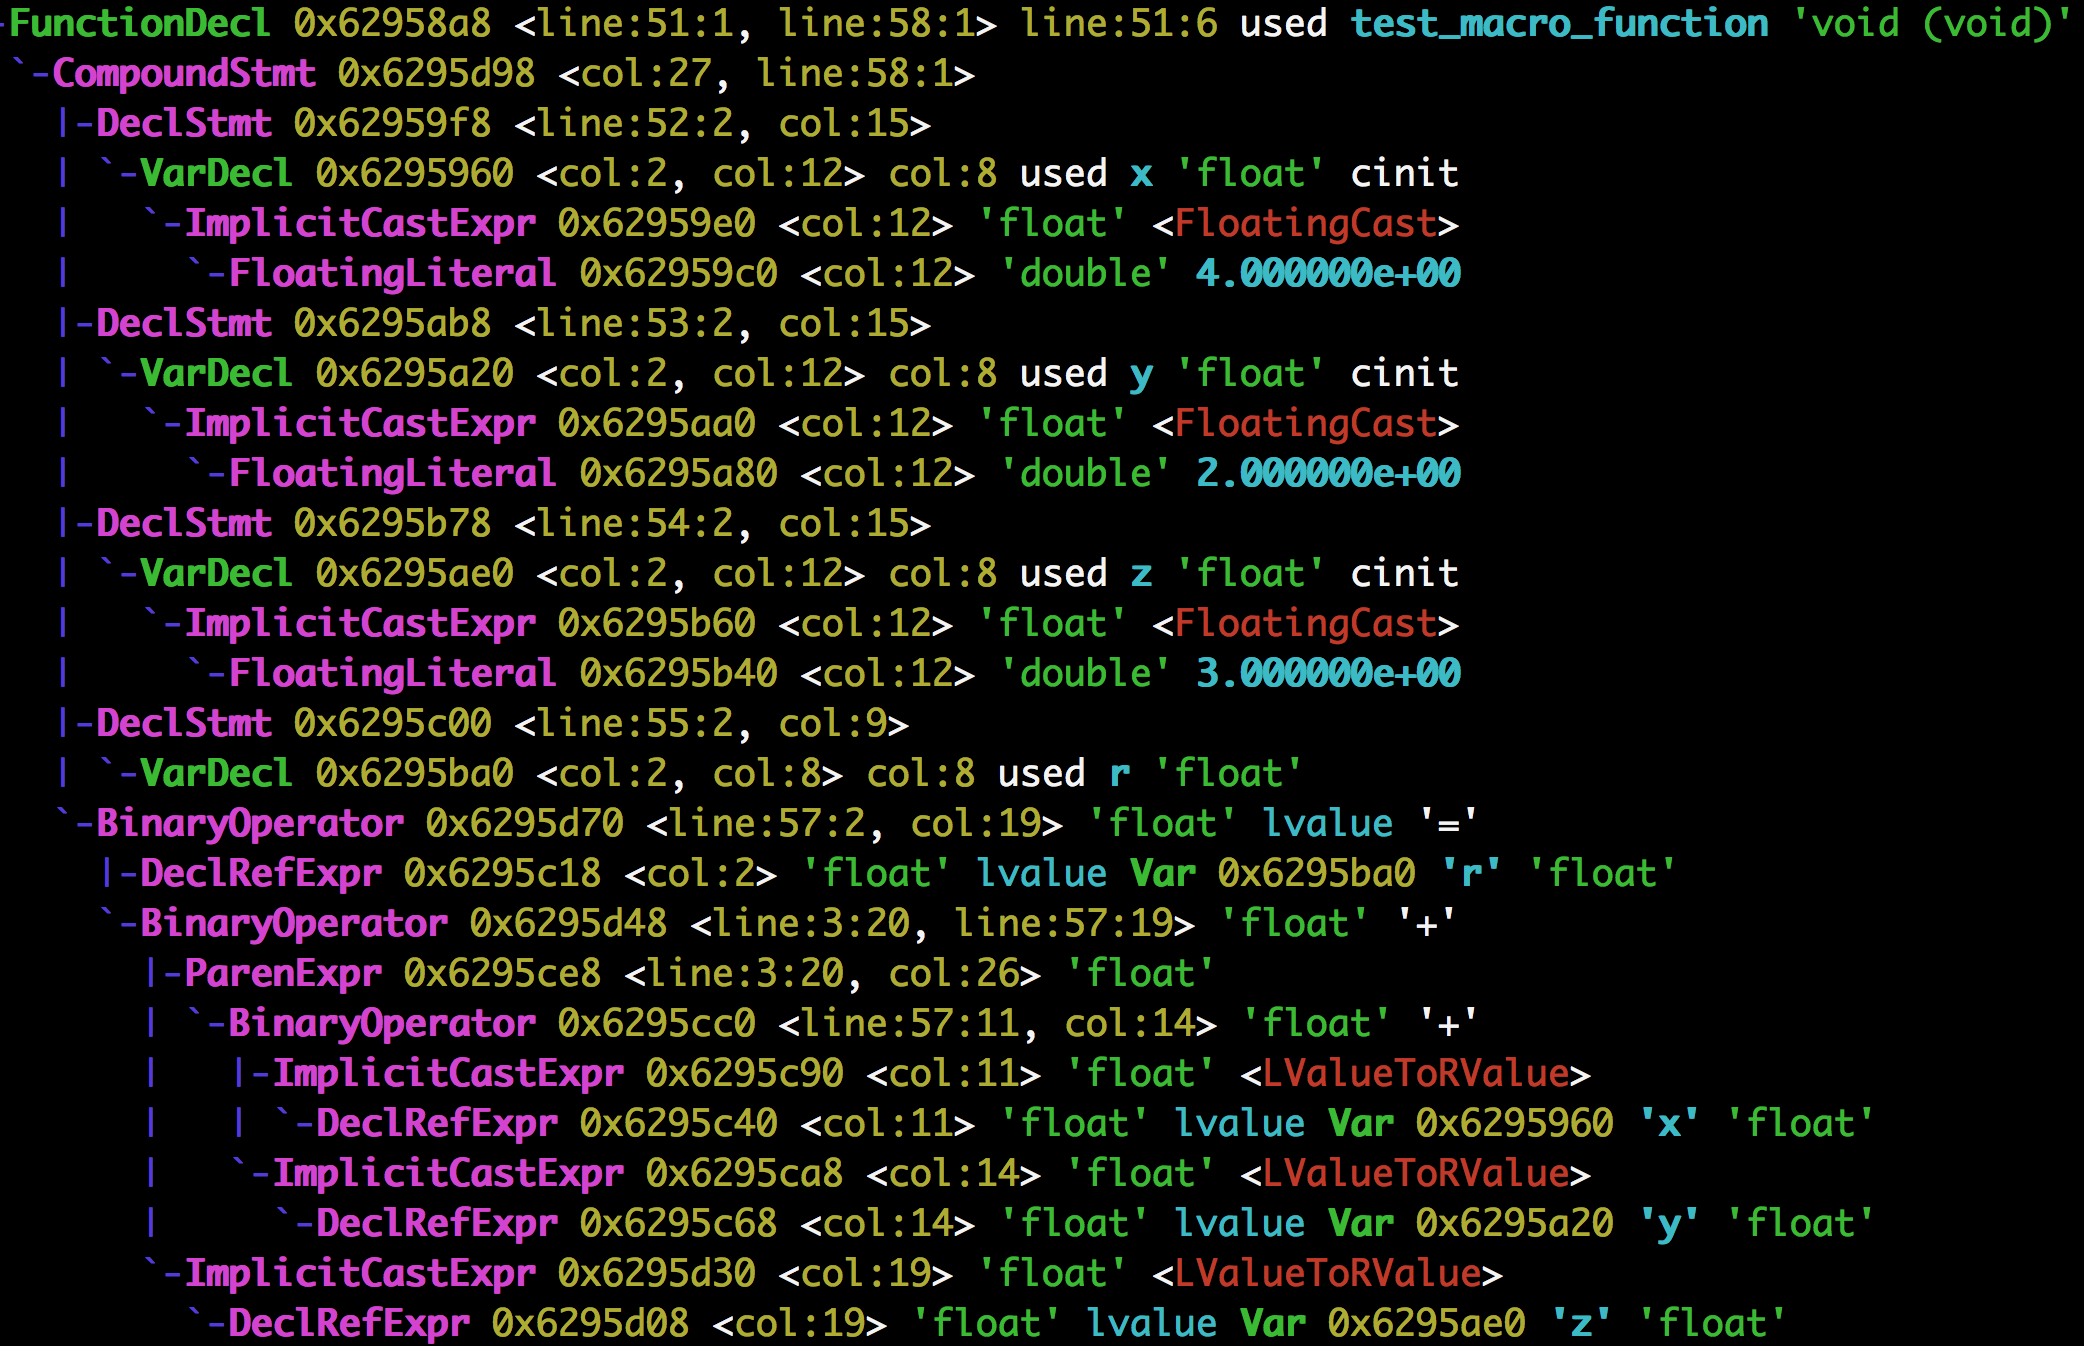
\includegraphics[width=15cm]{ast-sample.png}
\centering
\caption{IIDEAA's Execution Flow}
\end{figure}
~\\
A typical run of the framework consists of the following step: At the beginning, the user will provide to Chimera the original C/C++ source code  and the Approximate Operator that IIDEAA supports along with functions to test Approximate Computing on. At the next step, Chimera will try to mutate the source code with respect to the provided Operator, then proceed with a syntax check to ensure the mutation is successful. After that, Bellerophon will execute various version of the mutated source code by altering the mutator configuration, thus finding the best approximated version of the program. Criterion that can dictate which is the best configuration are how the error function (which calculate how much the approximated result deviate from the precise one), error threshold, and reward/penalty functions are defined. \\
~\\
The whole framework and running environment is publicly available at: \url{https://github.com/mariobarbareschi/iideaa-docker}

\subsection{Clang-Chimera}

Chimera was written in C/C++, based on the LLVM-Clang compiler. To be able to produce source-to-source mutation, Chimera exploits a few features of the said compiler. It inspects on the Clang's Abstract Syntax Tree which is a tree-based representation of the the source code. The tree contains nodes that symbolize the langague structure of a given source code. Moreover, a set of nodes will represent a specific patterns, which illustrates a peculiar structure of the source code. \\

%example of AST
\begin{figure}[H]
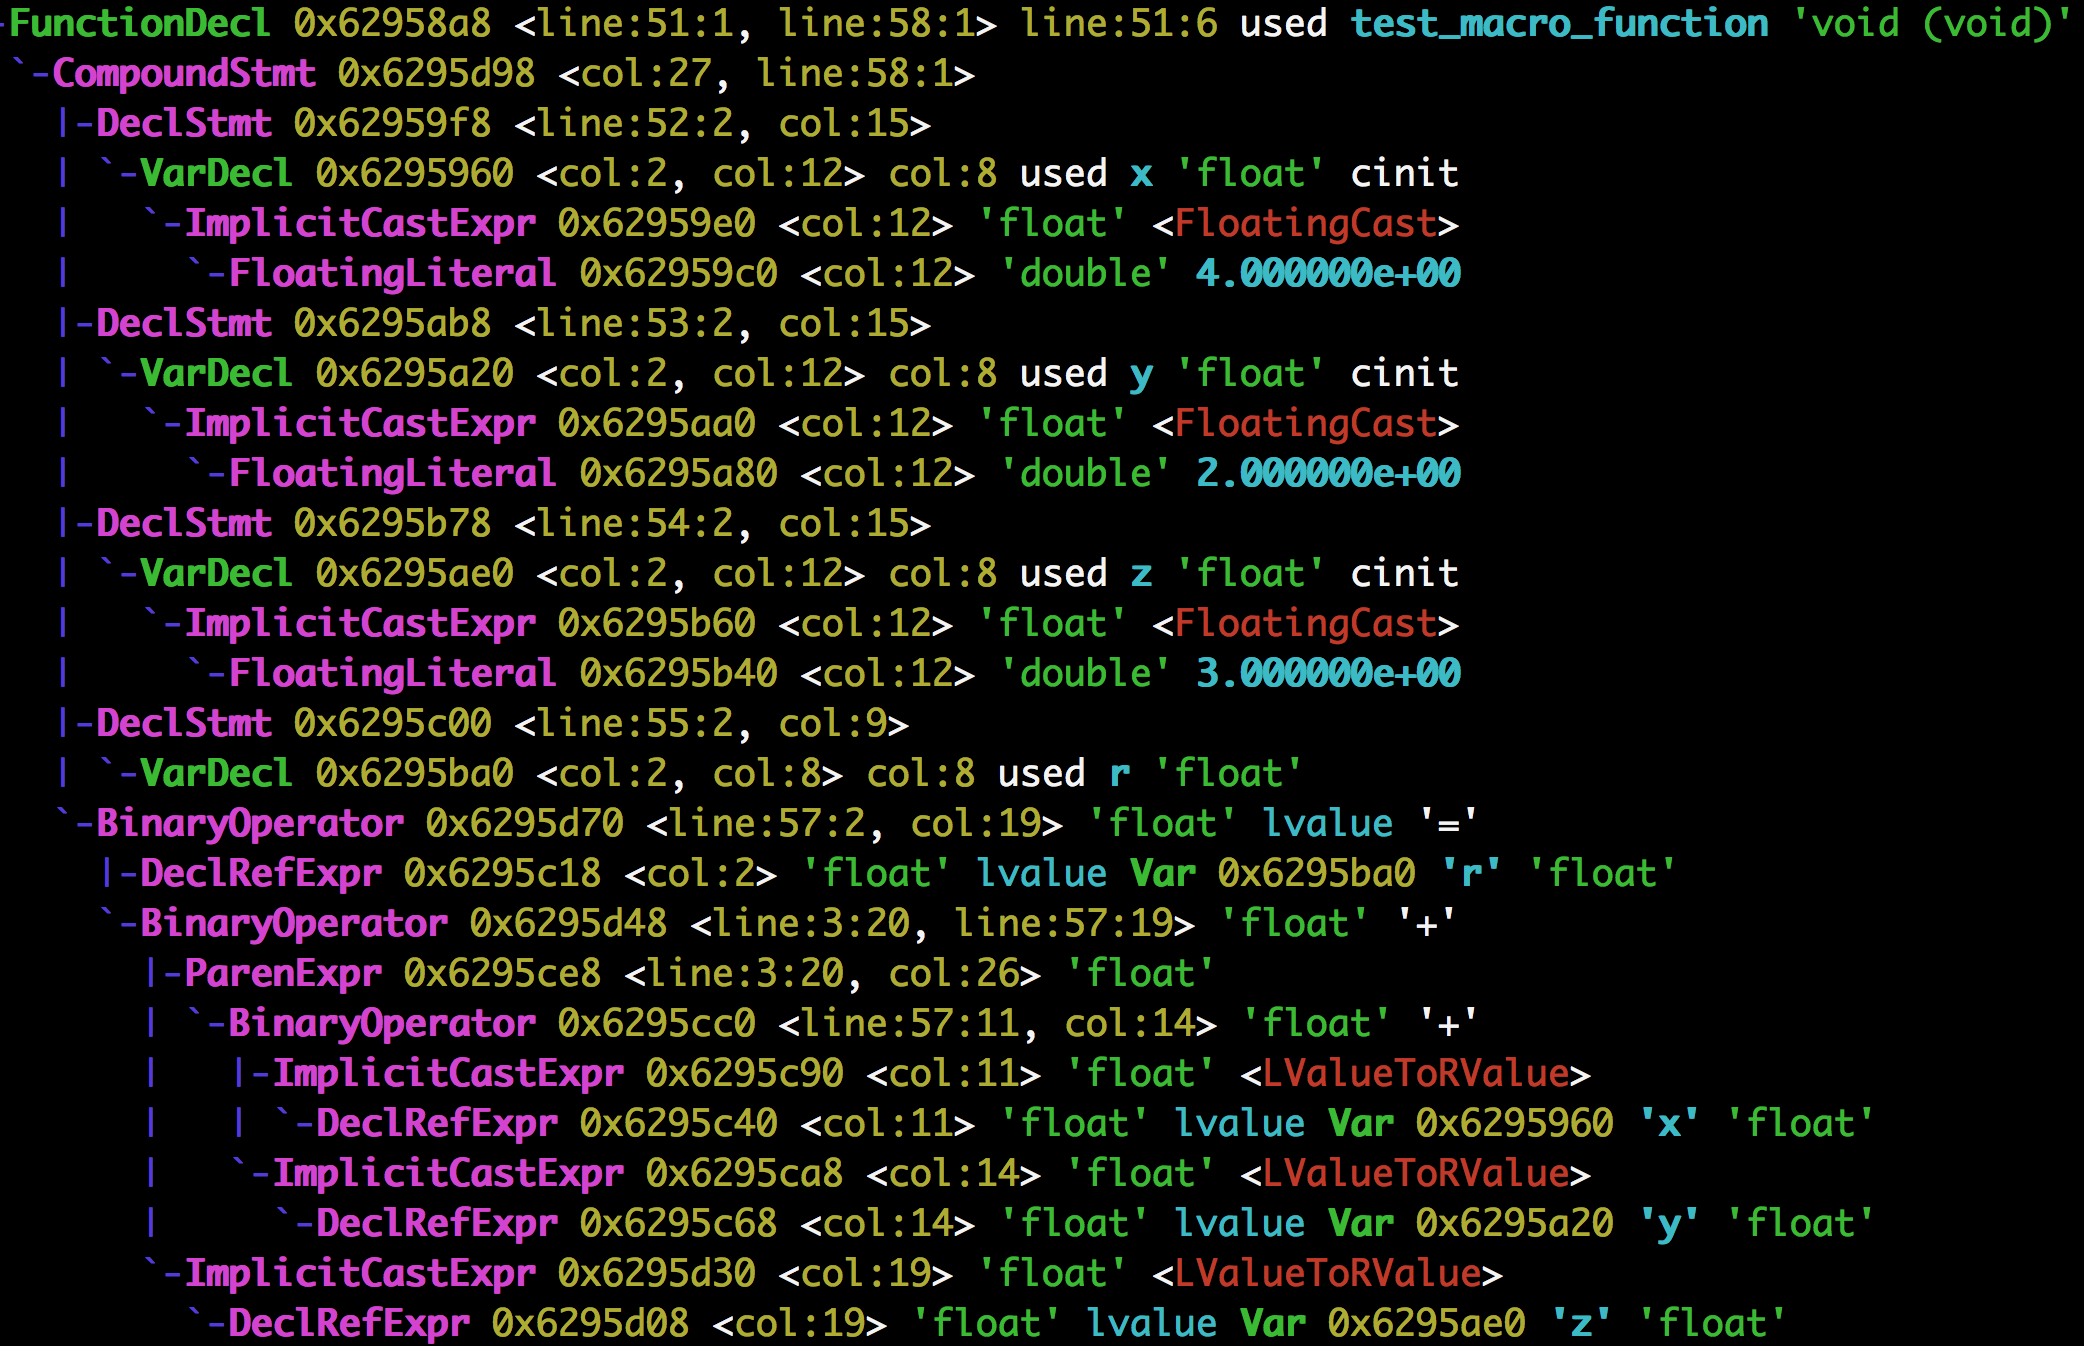
\includegraphics[width=15cm]{ast-sample.png}
\centering
\caption{Abstract Syntax Tree example of r = x + y + z in C++}
\end{figure}

By analyzing this Abstract Syntax Tree, Chimera is able to manipulate and mutate the source code with the help of 2 existing Clang API classes: \textit{ASTMatcher} and \textit{Rewriter}. With \textit{ASTMatcher}, Chimera is able to identify which nodes to mutate based on the given mutator. After all desired nodes have been found, \textit{Rewriter} will try to apply the mutation ~\cite{iideaa}. \\
~\\

\subsection{Bellerophon}

Bellerophon takes the mutated files and mutator configurations created by Chimera as input to explore all the different possibilities based on the parameters given by the user. To exploring each possibility, Bellerophon executes the mutated application based on the corresponding configuration and estimates their performance by a set of Fitness Functions. The definition of these Fitness Functions, generally include error(accuracy loss) and reward functions, should be defined by the user so that Bellerophon can function properly. The best configurations are those that satisfy the trade-off threshold between performance and accuracy loss ~\cite{iideaa}. \\
~\\
Bellerphon takes advantages of some features of the following tools. First, it uses the ParadisEO framework, which is a metaheuristics software consisting of many evolutionary algorithm, to effectively explore approximate variants of the mutated source code and configuration. Secondly, to reduce execution time, Bellerophon uses LLVM's Just-In-Time compiler which enables the ability to translate only what is mandatory for the mutated code (e.g. part of the code that was changed) to run ~\cite{iideaa}. Since there are many variants of the mutated program to execute, if the program has to re-compile for each time a new version is being tested, it will waste a lot of time. Just-In-Time compiler solve this problem by compiling section of code that are being use repeatly (e.g. code that was not mutated) once and interpreting the mutated sections \cite{JIT}. \\

\subsection{Current Challenges}
Since IIDEAA framework was developed recently, it is still far from perfect as it still lacks a core feautre. Currently, IIDEAA framework is only able to show which is the best configurations, which is inconvenient for the user. If Bellerophon results in many configurations, manually testing all of them will take time. Ideally, IIDEAA framework should have a tool to automatically generate the variants based on achieved results. Moreover, as it has not been tested widely, bugs may still occur when running the framework, either in Chimera or Bellerophon. \\

\section{State of The Art}

At the time of writing, a few frameworks have been developed to give the programmer the ability to declare which part of the program to apply Approximate Computing and how to do it. Example of this is by using compiler directive, the programmer can specify which loop in the source code to apply loop perforation technique. However, these frameworks has yet to provide the user features to explore through different possibilities of a Approximate Computing strategy, select and generate the best variants out of those prospects. \\
~\\
In the paper \cite{accept}, the author presented an automated compiler framework called ACCEPT. ACCEPT's goal is to provide a balance between automation and user's guidance. By introducing a new language extension for C/C++, ACCEPT provides programmers with C/C++ annotations that allow them to specify which part of the program to analyze and apply Approximation techniques. This was done by utilizing LLVM Intermediate Representation(IR) to modify the compiler to support the new language extension. The framework is also equipped with auto-tuning feature that try to find the best and provide feedback to the user. \\
~\\
Proposed in \cite{react}, REACT framework is an extension to ACCEPT that allow users to rapidly analyze Approximate Computing technique and assest the efficiency-accuracy trade-off produced by the technique. The framework contains 3 main part: an application profiler to instructions into categories, an energy model that estimate energy consumption based on the said categories and a quality model which extends ACCEPT and validate the quality of the approximation. \\
~\\
Precimonious, introduced in \cite{Precimonious}, is another framework that utilized LLVM-IR in order to conduct Approximate Computing investigation on floating-point data type through the mean of adding annotation and specifying the constraint of loss in accuracy. By doing so, the software will search for the configuration that can apply to the annotated code section, and further tune the precision based on the requirement. \\